%%%%%%%%%%%%%%%%%%%%%%%%%%%%%%%%%%%
%%  Webcam
%%%%%%%%%%%%%%%%%%%%%%%%%%%%%%%%%%%
\section{Webcam-Steuerung}
Zur Wetterstation Arbon gehört eine schwenk- und zoombare Webcam. Diese ist über ein Applikations-Plugin in die Webseite integriert. In der Titelleiste sind zusätzlich die wichtigsten Wetterdaten aufgeführt, wobei die Einheit der Windgeschwindigkeit jeweils alle dreissig Sekunden zwischen km/h und Knoten wechselt. Die Webseite der Webcam ist in Abbildung \ref{img:warteschlange} links dargestellt.

\begin{figure}[h]
	\centering
	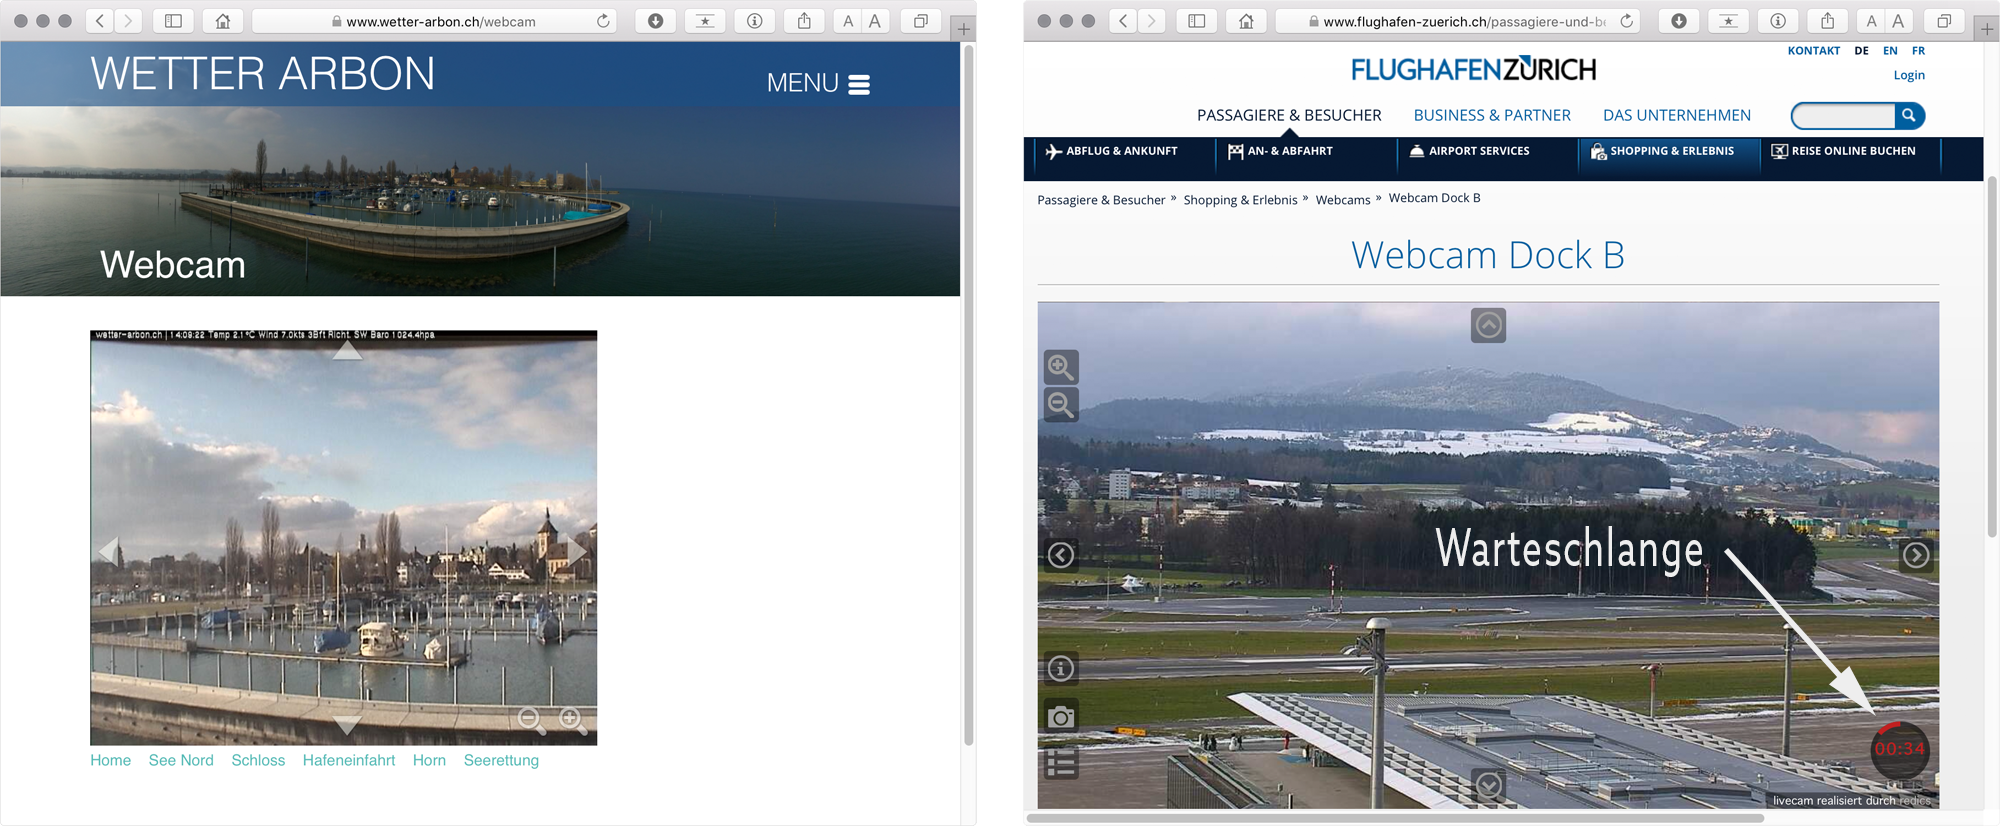
\includegraphics[width=1\linewidth]{img/warteschlange}
	\caption{Webcam Arbon und Beispiel einer Warteschlange}
	\label{img:warteschlange}
\end{figure}


% Warteschlange
\subsection{Warteschlange für Webcam-Steuerung}
Der Benutzer hat die Möglichkeit, die Webcam nach oben/unten und nach links/rechts zu bewegen. Sechs voreingestellte Positionen stehen als Shortlinks zur Verfügung. Diese Positionen sind in der betriebseigenen Software der Webcam konfigurierbar.
\newline

\noindent
%\subsection*{Problem}
Die Möglichkeit der Webcam-Steuerung übers Web ist zwar sehr attraktiv, hat aber auch seine Nachteile. Zum Beispiel wenn mehrere Personen gleichzeitig auf die Webcam zugreifen. Zur Zeit ist es so, dass die HTTP-Request der Reihe nach abgearbeitet werden. Es ist also möglich, dass sich die Benutzer gegenseitig in der Bedienung stören, was unter Umständen recht mühsam ist. 
\newline

\noindent
%\subsection*{Lösungsansatz}
Das Prinzip der Warteschlange kann hier Abhilfe schaffen. Jeder Benutzer erhält für eine bestimmte Zeit den alleinigen Zugriff auf die Steuerung der Webcam. Eine solche Lösung setzt zum Beispiel der Flughaben Zürich\footnote{ \url{https://www.flughafen-zuerich.ch/passagiere-und-besucher/shopping-und-erlebnis/webcams/webcam-dock-b}} ein, wie in Abbildung \ref{img:warteschlange} rechts dargestellt.



% Zoom
\subsection{Positionsabhängige Zoombeschränkung}
In der betriebseigenen Software der Webcam lassen sich viele Parameter konfigurieren, unter anderem der Zoomfaktor. 
\newline

\noindent
%\subsection*{Problem}
Das Problem ist, dass der Zoomfaktor nur allgemein eingestellt werden kann, das heisst die Beschränkung gilt immer, egal ob die Kamera auf eine Wohnung zeigt oder auf den See hinaus. Aus Persönlichkeitsschutz-Gründen musste deshalb der Zoomfaktor auf die 4-fache Vergrösserung limitiert werden, möglich wäre aber eine 216-fache Vergrösserung. Daraus wird deutlich, dass die Webcam eigentlich ein viel grösseres Potential hätte.
\newline

\noindent
%\subsection*{Lösungsansatz}
Die Idee ist nun, die Limitierung des Zooms so zu programmieren, dass diese möglichst dynamisch ist. Das heisst, dass je nach Position die Zoom-Limitierung ändert. Der Zoom soll vor allem auf den See hinaus in vollem Umfang genutzt werden können. Zudem darf die Funktion nicht umgangen werden können.


